%%%%%%%%%%%%%%%%%%%%%%%%%%%%%%%%%%%%%%%%%%%%%%%%%%%%%%%%%%%%%%%%%%%%%
% LaTeX Template: Project Titlepage Modified (v 0.1) by rcx
%
% Original Source: http://www.howtotex.com
% Date: February 2014
% 
% This is a title page template which be used for articles & reports.
% 
% This is the modified version of the original Latex template from
% aforementioned website.
% 
%%%%%%%%%%%%%%%%%%%%%%%%%%%%%%%%%%%%%%%%%%%%%%%%%%%%%%%%%%%%%%%%%%%%%%

\documentclass[12pt]{report}
\usepackage[a4paper]{geometry}
\usepackage[myheadings]{fullpage}
\usepackage{fancyhdr}
\usepackage{lastpage}
\usepackage{graphicx, wrapfig, subcaption, setspace, booktabs}
\usepackage[T1]{fontenc}
\usepackage[font=small, labelfont=bf]{caption}
\usepackage{fourier}
\usepackage[protrusion=true, expansion=true]{microtype}
\usepackage[english]{babel}
\usepackage{sectsty}
\usepackage{url, lipsum}
\usepackage{listings}
\usepackage{color}
\definecolor{codegreen}{rgb}{0,0.6,0}
\definecolor{codegray}{rgb}{0.5,0.5,0.5}
\definecolor{codepurple}{rgb}{0.58,0,0.82}
\definecolor{backcolour}{rgb}{0.95,0.95,0.92}
\usepackage{url}
\DeclareUrlCommand\r{%
  \renewcommand\UrlFont{\ttfamily\color{blue}}%
  \renewcommand\UrlLeft{\uline\bgroup}%
  \renewcommand\UrlRight{\egroup}}
\lstdefinestyle{mystyle}{
    backgroundcolor=\color{backcolour},   
    commentstyle=\color{codegreen},
    keywordstyle=\color{magenta},
    numberstyle=\tiny\color{codegray},
    stringstyle=\color{codepurple},
    basicstyle=\footnotesize,
    breakatwhitespace=false,         
    breaklines=true,                 
    captionpos=b,                    
    keepspaces=true,                 
    numbers=left,                    
    numbersep=5pt,                  
    showspaces=false,                
    showstringspaces=false,
    showtabs=false,                  
    tabsize=2
}
\lstset{style=mystyle}
\usepackage{graphicx}
\graphicspath{ {images/} }


\newcommand{\HRule}[1]{\rule{\linewidth}{#1}}
\onehalfspacing
\setcounter{tocdepth}{5}
\setcounter{secnumdepth}{5}

%-------------------------------------------------------------------------------
% HEADER & FOOTER
%-------------------------------------------------------------------------------
\pagestyle{fancy}
\fancyhf{}
\setlength\headheight{15pt}
\fancyhead[L]{Senior Design Team 3}
\fancyhead[R]{Wright State University}
\fancyfoot[R]{Page \thepage\ of \pageref{LastPage}}
%-------------------------------------------------------------------------------
% TITLE PAGE
%-------------------------------------------------------------------------------

\begin{document}

\title{ \normalsize \textsc{Software Guide}
		\\ [2.0cm]
		\HRule{0.5pt} \\
		\LARGE \textbf{\uppercase{Intracranial Pressure Waveform Generator}}
		\HRule{2pt} \\ [0.5cm]
		\normalsize \today \vspace*{5\baselineskip}}

\date{}

\author{
		Senior Design Team 3 \\
		Wright State University \\
		Department of Biomedical, Industrial, and Human Factors Engineering }

\maketitle
\tableofcontents
\newpage

%-------------------------------------------------------------------------------
% Section title formatting
\sectionfont{\scshape}
%-------------------------------------------------------------------------------

%-------------------------------------------------------------------------------
% BODY
%-------------------------------------------------------------------------------


\listoffigures
\newpage

\lstlistoflistings
\newpage


\section*{Raspberry Pi Setup}
\addcontentsline{toc}{section}{Raspberry Pi Setup}
\subsection*{1. Hardware}
Raspberry Pi 3 \newline Pi Cobbler \newline Adafruit Digital Analog Converter (DAC) \newline 32 GB or more microSD Card \newline Keyboard \newline Computer Mouse \newline Wireless HDMI
\subsection*{2. Software Installation}
\subsubsection*{NOOBS Install}
 We installed NOOBS as the operating system installer. A microSD card with at least 32 GB of storage is required. The set up was as follows:
 \newline 1. Insert microSD into computer \newline 2. Go to \url{https://www.raspberrypi.org/downloads/noobs/} and download the NOOBS zip file \newline 3.  Extract the zip flie onto the microSD \newline 4. Eject the microSD and insert into the Raspberry Pi \nweline 5. Power the Raspberry Pi on. The first screen that will appear select Raspbian and install \newline 6. The Pi will now reboot and after it has power back on the Raspberry Pi is now ready for use 
\newline\newline Set up: 
\url{https://www.youtube.com/watch?v=wvxCNQ5AYPg}
\subsection*{3. Login Credentials}
\newline The username is "pi" -- all lowercase
\newline The password is "ICP" -- all capitalized letters
\subsection*{4. Package Installation}
\newline The process for installing any python packages should be done as follows from inside the terminal: \newline 1. Run "sudo apt update" through the terminal before installing new software packages. This will ensure that all packages are the lastest version and avoid any versioning issues with newer installed packages. 
\newline 2. Type "sudo pip3 install xxxxxx" where xxxxxx is the name of the package with which you wish to install. \newline 3. This will not include all necessary packages so if one of them doesn't work using "sudo pip3 install" then it is acceptable to use "sudo apt-get install python3-xxxxxx".
\subsubsection*{Viewing installed packages}
To check if a package is installed type into the terminal "dpkg -l | grep <keyword>", where <keyword> is (part of) the name of the package you are interested in finding. For example, searching "dpkg -l | grep nvidia" will list all installed packages with "nvidia" in the name or description. This method will not work for meta-packages or repositories, though it will work for most cases. You can check where a package is installed by typing "sudo dpkg -S packagename".
\subsubsection*{The packages that are required for our system are as follows:}
\newline1. Adafruit MCP4275
\newline
    Used for the DAC chip. Install was set up using: 
    \newline \url{https://learn.adafruit.com/mcp4725-12-bit-dac-with-raspberry-pi}
    \newline
\newline 2. Guizero
\newline
    Used for the creation of the Graphical User Interface (GUI).
    \newline
\newline 3. ScipPy
\newline
    contains modules for optimization, linear algebra, integration, interpolation, special functions, FFT, signal and image processing, ODE solvers and other tasks.
    \newline
\newline4. Numpy
\newline
    Used for multi-dimensional arrays and matrices, along with a large collection of high-level mathematical functions.
    \newline
\newline 5.I2C
\newline
    A bus that allows a connection between the pi and wiring through the GPIO pins. Setup was done through:
\newline  
\url{https://learn.sparkfun.com/tutorials/raspberry-pi-spi-and-i2c-tutorial/all}
\newline
\newline6. GPIO
\newline
    These are the pins that the connects the code to the DAC chip. This connection is done through the Pi Cobbler. This software allows you to pick the pin the signal will come out of. Setup for this was done through: 
\newline
\url{https://www.raspberrypi-spy.co.uk/2012/05/install-rpi-gpio-python-library/}

\section*{Troubleshooting}
\addcontentsline{toc}{section}{Troubleshooting}
\subsection*{White Bar Across Left Half of Screen}
If a white bar appears across the left side of the screen and cannot click on the menu then follow these steps:
\newline Control + Alt + F1
\newline username: pi, password: ICP
\newline sudo rm -r ~/.config/lxpanel
\newline startx

\subsection*{HDMI Will Not Display}
\newline The Raspberry Pi must first be plugged in before the HDMI can be plugged in. 

\subsection*{Code Will Not Execute Because Pi Cannot Discover I2C Bus Location}
\newline Chances are that the DAC chip has fried and needs to be replaced. If this is not the case, check to see which I2C location the Pi is trying to output the code by typing into the terminal "i2cdetect -y 1".

\subsection*{Pi Will Not Turn On}
\newline Check to see what color is being displayed by the LED. If only red is showing, the SD card is either inserted incorrectly or corrupted. It should have a red LED with a green LED that intermittently blinks. 
\subsection*{Board Goes Off Intermittently}
\newline This is due to the power. Make sure that the Pi is plugged into a power supply that outputs 5V and 2.5A.
\section*{Digital Analog Converting Software}
\addcontentsline{toc}{section}{Digital Analog Converting Software}
The MCP4725 is a 12-bit DAC chip that converts the digital signal into an analog output to be properly displayed on the ProPAQ patient monitor. Determining what output voltage is given is. The voltage that is output is determined by the following equation: 
\newline
$$V_{out} = \frac{(V_{cc} * Bit \quad Value)}{4096}$$
\newline
The $V_{cc}$ is the output voltage from the Raspberry Pi. The system has a $V_{cc}$ of 5V. There are two sources from the Raspberry Pi, 3.3V and 5V. The 5V source output higher resolution waveform and that is why that source was chosen. 
\section*{Frequency Calculation}
In order for the ICP waveform to have the same time synchronization as the EKG waveform, they must have the same frequency. This is calculated using the following equation: 
$$Length \quad  of \quad  Waveform = e^{\frac{-(BPM + 193.74)}{54.91}}$$
\newline
This equation can be seen in each of the waveform model files (ex. modelone.py). 
\addcontentsline{toc}{section}{Frequency Calculation}
\section*{Computer Application}
\addcontentsline{toc}{section}{Computer Application}



\begin{figure}[h!]
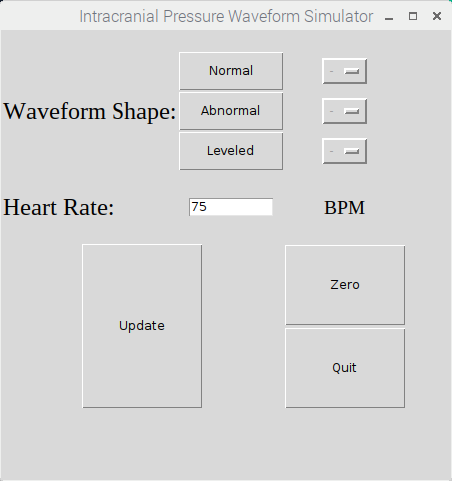
\includegraphics[width=10cm]{GUI}
\centering
\label{fig:figure1}
\caption{GUI}
\end{figure}
\newline
\newline
\lstset{language=Python}
\lstset{frame=lines}
\lstset{caption={Calibration}, captionpos=t}
\lstset{label={lst:code_direct}}
\lstset{basicstyle=\footnotesize}
\lstset{caption={Gui Code}}
\newpage
\begin{lstlisting}
from guizero import App, Box, Text, Slider, TextBox, ButtonGroup, PushButton, CheckBox, MenuBar
import subprocess
import signal
import os
import sys

#Pulled in the necessary tools to create the GUI

class MyGUI:
    rate = 60 #Initialize Heart Rate at 65 
    def __init__(self, master):
        self.master = master
        self.menubar = MenuBar(master,
                  toplevel=["File", "Help"],
                  options=[
                      [ ["Exit", self.exit ] ],
                      [["Waveform Shape", self.exit ],["Heart Rate", self.exit],["ICP Value", self.exit]]
                      ])
       #Creates the application window

        self.ICPmessage = Text(master, size=18, text="ICP:", grid=[0,0], align="left", font="Times")
        self.ICPstart = Text(master, text="0 mmHg", grid=[1,0], font="Times")
        self.ICPslider = Slider(master, command=self.ICPslider_changed, start=0, end=30, grid=[2,0])
        self.ICPend = Text(master, text="30 mmHg", grid=[3,0], font="Times")
        #Creates the ICP subtitle and slider

        self.ICPval = TextBox(master, grid=[2,1], text=0)
        self.ICPunit = Text(master, size=15, text='mmHg', grid=[3,1], font="Times")
        #Creates the ICP textbox to allow for typed input

        self.space1 = Text(master, text=" ", grid=[0,2])
        #Creates space between ICP and Waveform Shape

        self.Shapemessage1 = Text(master, size=18, text="Waveform Shape:", grid=[0,3,1,2], align="left", font="Times")
        self.Override = CheckBox(master, text="Automatic Shape", command=self.show_choices, grid=[2,3,2,1], align="left")
        self.Override.toggle()
        self.ShapeOverride = ButtonGroup(master, options=["Normal", "Leveled","Abnormal"], selected="Normal", grid=[2,4,1,2], command=self.modelone)
        self.ShapeOverride = ButtonGroup(master, options=["Normal", "Leveled","Abnormal"], selected="Leveled", grid=[2,4,1,2], command=self.modeltwo)
        self.ShapeOverride = ButtonGroup(master, options=["Normal", "Leveled","Abnormal"], selected="Abnormal", grid=[2,4,1,2], command=self.modelthree)
        self.ShapeOverride = ButtonGroup(master, options=["Normal", "Leveled","Abnormal"], selected=0, grid=[2,4,1,2], command= self.modelone)

        self.ShapeOverride.disable()
        #Creates the Waveform Shape subtitle and "Button Group"
        #By default, shape is automatically chosen, but, if box is unchecked, user is able to override the defaulted shape

        self.space2 = Text(master, text=" ", grid=[0,6])
        #Creates space between Waveform Shape and Heart Rate

        self.HRmessage = Text(master, size=18, text="Heart Rate:", grid=[0,8], align="left", font="Times")
        self.HRstart = Text(master, text="0 BPM", grid=[1,8], font="Times")
        self.HRslider = Slider(master, command=self.HRslider_changed, start=0, end=300, grid=[2,8])
        self.HRend = Text(master, text="300 BPM", grid=[3,8], font="Times")
        #Creates the HR subtitle and slider

        self.HRval = TextBox(master, grid=[2,10], text=self.rate)
        self.HRunit = Text(master, size=15, text="BPM", grid=[3,10], font="Times")
        #Creates the HR textbox to allow for typed input

        self.space3 = Text(master, text=" ", grid=[0,11], font="Times")
        #Creates space between Heart Rate and the Update Button

        self.button = PushButton(master, command=self.update_value, width="12", height="2", text="Update", grid=[0,12,12,6], align="bottom")
        #Creates an Update Button that updates the inputed information and exports the user-inputs to the next part of the program
        self.when_clicked = self.update_value
        self.when_mouse_enters = self.update_value
        #If cursor is clicked or moved elsewhere, the slider and textbox are synced
        self.button = PushButton(master, command=self.calibration, width="8", height="2", text="Zero", grid=[0,12,1,1], align="bottom")

        self.pid = -1 #Initialize process id


    #Launches the function for modelone , Normal ICP, in a seperate python process and obtains the process ID
    def modelone(self):
        self.done()
        self.process = subprocess.Popen('python modelone.py {}'.format(self.rate), shell=True, preexec_fn=os.setsid)
        self.pid = self.process.pid

    #Launches the function for modeltwo , Leveled ICP, in a seperate python process and obtains the process ID    
    def modeltwo(self):
        self.done()
        self.process = subprocess.Popen('python modeltwo.py {}'.format(self.rate), shell=True, preexec_fn=os.setsid)
        self.pid = self.process.pid

    #Launches the function for modelthree, Abnormal ICP, in a seperate python process and obtains the process ID    
    def modelthree(self):
        self.done()
        self.process = subprocess.Popen('python modelthree.py {}'.format(self.rate), shell=True, preexec_fn=os.setsid)
        self.pid = self.process.pid

    def calibration(self):
        self.done()
        self.process = subprocess.Popen('python calibration.py', shell=True, preexec_fn=os.setsid)
        self.pid = self.process.pid

    def ICPslider_changed(self):
        self.done()
        self.ICPval.value = self.ICPslider.value

    def show_choices(self):
        self.done()
        if self.Override.value == 0:
            self.ShapeOverride.enable()
            self.command = self.modelone
        if self.Override.value == 1:
            self.ShapeOverride.disable()
            self.ShapeOverride.value = 0

    #If the "Automatic Shape" is unchecked, the user is able to override the selected shape and choose a new one

    def HRslider_changed(self):
        self.done()
        self.HRval.value = self.HRslider.value
        #self.rate = self.HRslider.value
        self.rate = self.HRval.value
        self.rate = self.HRslider.value

    #If the Heart Rate (HR) slider is changed, the value in the textbox is also changed

    def update_value(self):
        if self.ICPval.value == "":
            self.ICPval.value=0
        if self.HRval.value == "":
            self.HRval.value=0
        self.ICPslider.value = self.ICPval.value
        #self.HRslider.value = self.HRval.value
        self.ICPval.value = self.ICPslider.value
        self.rate = self.HRslider.value

     #Kills the process that is currently running
    def done(self):
        if self.pid > 0:
            try:
                os.killpg(os.getpgid(self.pid), signal.SIGTERM)
                self.pid = -1
            except ProcessLookupError:
                pass


    #closes out of the GUI and kills any running processes    
    def exit(self):
        self.done()
        self.master.destroy()

#If cursor clicks something or moves elsewhere or the Update Button is clicked, the value entered in the textbox is used to set the slider value
#The textbox value is set to the slider value again in the event that two values exceeding the range are inputed consecutively 
root = App(title="Intracranial Pressure Waveform Simulator", width=450, height=350, layout="grid")
#app=App.display()
#Pulls up the GUI
my_gui = MyGUI(root)
root.display()
#Creates the application window
\end{lstlisting}

\section*{Waveform Codes}
\addcontentsline{toc}{section}{Waveform Codes}
The waveform codes each rely on a different MATLAB file which contains a graph of the specfied waveform. It then converts each point on the MATLAB plot into bit values that the DAC will recognize and be able to output the specified voltage. \newline\newline The Calibration Code is used to zero the ProPAQ. This should be done before running the simulation just to initialize the system. This should be run before zeroing the probe on the ProPAQ. The process is as follows: \newline 1. Start the GUI and press the zero button \newline 2. Zero the probe on the ProPAQ and change the scaling from 30 to -30 \newline execute the desired waveform, ICP value, and heart rate 
\lstset{language=Python}
\lstset{frame=lines}
\lstset{caption={Calibration}, captionpos=t}
\lstset{label={lst:code_direct}}
\lstset{basicstyle=\footnotesize}
\begin{lstlisting}
#Imports to Recognize the Dac on the Raspberry Pi
import Adafruit_MCP4725

dac = Adafruit_MCP4725.MCP4725()


zero = 300;
zero = int(zero)
dac.set_voltage(zero) #Set the output Voltage to Zero
\end{lstlisting}

\lstset{caption={Normal Waveform}, captionpos=t}

\begin{figure}[h!]
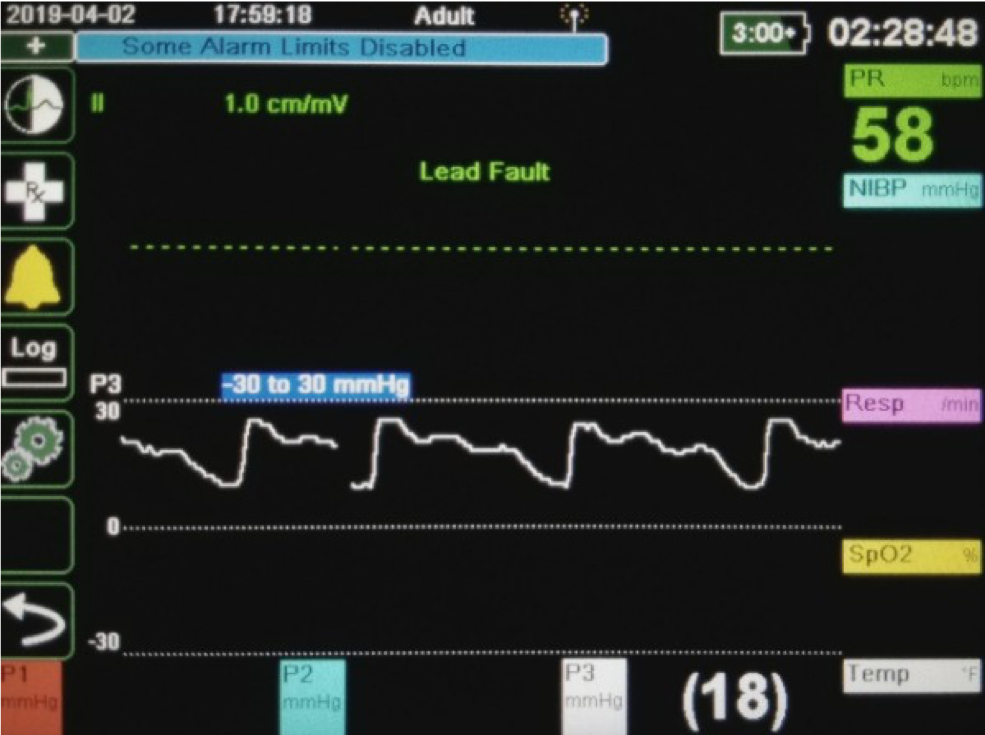
\includegraphics[width = 10cm]{Normal.png}
\centering
\caption{Normal Waveform}
\end{figure}

\newpage
\begin{lstlisting}
from scipy import io
import numpy as np
import time
import sys
import math
import Adafruit_MCP4725

#Imports to Recognize the DAC chip on the Pi
dac = Adafruit_MCP4725.MCP4725()

#Initialize the function variables
first_arg = sys.argv[1]

def modelone(intvalue = first_arg): #first_arg
    intvalue = int(intvalue)
    mat = io.loadmat('modelonescale.mat'); #Load the Waveform model matrix
    y_value = mat['interpoalteddatay'];
    y_value = np.transpose(y_value);
    new_value = np.zeros(y_value.shape) #Create a Zero Matrix to fill with Voltage Values


    #Conversion table between the model and the Voltages
    for jj in range(len(y_value)):
        if y_value[jj] == 1:
            new_value[jj] = 3900
        elif y_value[jj] == 2:
            new_value[jj] = 3550
        elif y_value[jj] == 3:
            new_value[jj] = 3350
        elif y_value[jj] == 4:
            new_value[jj] = 3200
        elif y_value[jj] == 5:
            new_value[jj] = 2950
        elif y_value[jj] == 6:
            new_value[jj] = 2820
        elif y_value[jj] == 7:
            new_value[jj] = 2700
        elif y_value[jj] == 8:
            new_value[jj] = 2620
        elif y_value[jj] == 9:
            new_value[jj] = 2540
        elif y_value[jj] == 10:
            new_value[jj] = 2460
        elif y_value[jj] == 11:
            new_value[jj] = 2380
        elif y_value[jj] == 12:
            new_value[jj] = 2300
        elif y_value[jj] == 13:
            new_value[jj] = 2240
        elif y_value[jj] == 14:
            new_value[jj] = 2190
        elif y_value[jj] == 15:
            new_value[jj] = 2145
        elif y_value[jj] == 16:
            new_value[jj] = 2100
        elif y_value[jj] == 17:
            new_value[jj] = 2055
        elif y_value[jj] == 18:
            new_value[jj] = 2020
        elif y_value[jj] == 19:
            new_value[jj] = 1985
        elif y_value[jj] == 20:
            new_value[jj] = 1950
        elif y_value[jj] == 21:
            new_value[jj] = 1920
        elif y_value[jj] == 22:
            new_value[jj] = 1894
        elif y_value[jj] == 23:
            new_value[jj] = 1870
        elif y_value[jj] == 24:
            new_value[jj] = 1848
        elif y_value[jj] == 25:
            new_value[jj] = 1828
        elif y_value[jj] == 26:
            new_value[jj] = 1811
        elif y_value[jj] == 27:
            new_value[jj] = 1794
        elif y_value[jj] == 28:
            new_value[jj] = 1779
        elif y_value[jj] == 29:
            new_value[jj] = 1764
        elif y_value[jj] == 30:
            new_value[jj] = 1751
        elif y_value[jj] == 31:
            new_value[jj] = 1735
           
    
    
    var = 1;
    
    X = math.exp(-(intvalue+193.74)/54.91)#Calculate Heart Rate
    new_value = new_value.flatten()

    #Output the Voltages to the Raspberry PI
    while var == 1:
        for val in new_value:
            val = int(val)
            dac.set_voltage(val)
            time.sleep(X)
if __name__ == "__main__":
    modelone()
\end{lstlisting}
\lstset{caption={Abnormal Waveform}, captionpos=t}
\begin{figure}[h!]
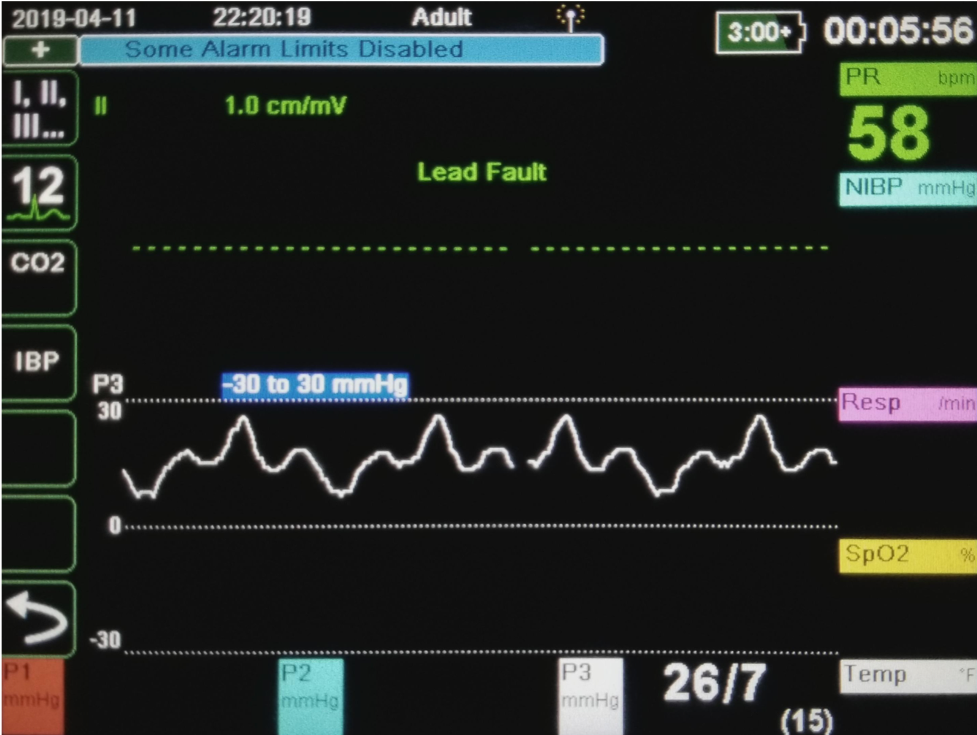
\includegraphics[width = 10cm]{Abnormal.png}
\centering
\caption{Abnormal Waveform}
\end{figure}
\newpage
\begin{lstlisting}
from scipy import io
import numpy as np
import time
import sys
import math
import Adafruit_MCP4725

#Imports to Recognize the DAC chip on the Pi
dac = Adafruit_MCP4725.MCP4725()
#Initialize the function variables
first_arg = sys.argv[1]

def modeltwo(intvalue = first_arg):
    intvalue = int(intvalue)
    mat = io.loadmat('modeltwoscale.mat'); #Load the Files
    y_value = mat['modeltwo'];
    y_value = np.transpose(y_value);
    new_value = np.zeros(y_value.shape)#Create a Zero Matrix to fill with Voltage Values
    
    #Conversion table between the model and the Voltages
    for jj in range(len(y_value)):
        if y_value[jj] == 1:
            new_value[jj] = 3900
        elif y_value[jj] == 2:
            new_value[jj] = 3550
        elif y_value[jj] == 3:
            new_value[jj] = 3350
        elif y_value[jj] == 4:
            new_value[jj] = 3200
        elif y_value[jj] == 5:
            new_value[jj] = 2950
        elif y_value[jj] == 6:
            new_value[jj] = 2820
        elif y_value[jj] == 7:
            new_value[jj] = 2700
        elif y_value[jj] == 8:
            new_value[jj] = 2620
        elif y_value[jj] == 9:
            new_value[jj] = 2540
        elif y_value[jj] == 10:
            new_value[jj] = 2460
        elif y_value[jj] == 11:
            new_value[jj] = 2380
        elif y_value[jj] == 12:
            new_value[jj] = 2300
        elif y_value[jj] == 13:
            new_value[jj] = 2240
        elif y_value[jj] == 14:
            new_value[jj] = 2190
        elif y_value[jj] == 15:
            new_value[jj] = 2145
        elif y_value[jj] == 16:
            new_value[jj] = 2100
        elif y_value[jj] == 17:
            new_value[jj] = 2055
        elif y_value[jj] == 18:
            new_value[jj] = 2020
        elif y_value[jj] == 19:
            new_value[jj] = 1985
        elif y_value[jj] == 20:
            new_value[jj] = 1950
        elif y_value[jj] == 21:
            new_value[jj] = 1920
        elif y_value[jj] == 22:
            new_value[jj] = 1894
        elif y_value[jj] == 23:
            new_value[jj] = 1870
        elif y_value[jj] == 24:
            new_value[jj] = 1848
        elif y_value[jj] == 25:
            new_value[jj] = 1828
        elif y_value[jj] == 26:
            new_value[jj] = 1811
        elif y_value[jj] == 27:
            new_value[jj] = 1794
        elif y_value[jj] == 28:
            new_value[jj] = 1779
        elif y_value[jj] == 29:
            new_value[jj] = 1764
        elif y_value[jj] == 30:
            new_value[jj] = 1751
        elif y_value[jj] == 31:
            new_value[jj] = 1735
            
    new_value = new_value.flatten()
    var = 2;
    X = math.exp(-(intvalue+193.74)/54.91) #Calculate Heart Rate

    #Output the Voltages to the Raspberry PI
    while var == 2:
        for val in new_value:
            val = int(val)
            dac.set_voltage(val)
            time.sleep(X)
if __name__ == "__main__":
    modeltwo()

\end{lstlisting}
\lstset{caption={Leveled Waveform}, captionpos=t}
\begin{figure}[h!]
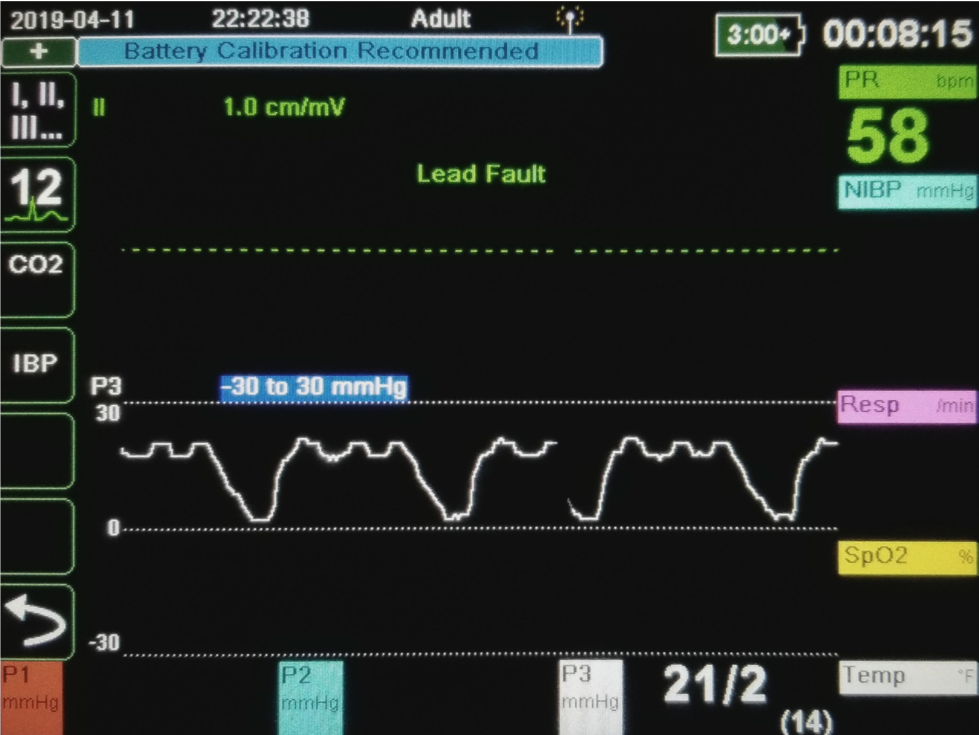
\includegraphics[width = 10cm]{Leveled.png}
\centering
\caption{Leveled Waveform}
\end{figure}
\newpage
\begin{lstlisting}
from scipy import io
import numpy as np
import time
import sys
import math
import Adafruit_MCP4725

#Imports to Recognize the DAC chip on the Pi
dac = Adafruit_MCP4725.MCP4725()
#Initialize the function variables
first_arg = sys.argv[1]

def modelthree(intvalue = first_arg):
    intvalue = int(intvalue)
    mat = io.loadmat('modelthreescaling.mat'); #Load the Waveform model matrix
    y_value = mat['modelthree'];
    y_value = np.transpose(y_value);
    new_value = np.zeros(y_value.shape) #Create a Zero Matrix to fill with Voltage Values

    #Conversion table between the model and the Voltages
    for jj in range(len(y_value)):
        if y_value[jj] == 1:
            new_value[jj] = 3900
        elif y_value[jj] == 2:
            new_value[jj] = 3550
        elif y_value[jj] == 3:
            new_value[jj] = 3350
        elif y_value[jj] == 4:
            new_value[jj] = 3200
        elif y_value[jj] == 5:
            new_value[jj] = 2950
        elif y_value[jj] == 6:
            new_value[jj] = 2820
        elif y_value[jj] == 7:
            new_value[jj] = 2700
        elif y_value[jj] == 8:
            new_value[jj] = 2620
        elif y_value[jj] == 9:
            new_value[jj] = 2540
        elif y_value[jj] == 10:
            new_value[jj] = 2460
        elif y_value[jj] == 11:
            new_value[jj] = 2380
        elif y_value[jj] == 12:
            new_value[jj] = 2300
        elif y_value[jj] == 13:
            new_value[jj] = 2240
        elif y_value[jj] == 14:
            new_value[jj] = 2190
        elif y_value[jj] == 15:
            new_value[jj] = 2145
        elif y_value[jj] == 16:
            new_value[jj] = 2100
        elif y_value[jj] == 17:
            new_value[jj] = 2055
        elif y_value[jj] == 18:
            new_value[jj] = 2020
        elif y_value[jj] == 19:
            new_value[jj] = 1985
        elif y_value[jj] == 20:
            new_value[jj] = 1950
        elif y_value[jj] == 21:
            new_value[jj] = 1920
        elif y_value[jj] == 22:
            new_value[jj] = 1894
        elif y_value[jj] == 23:
            new_value[jj] = 1870
        elif y_value[jj] == 24:
            new_value[jj] = 1848
        elif y_value[jj] == 25:
            new_value[jj] = 1828
        elif y_value[jj] == 26:
            new_value[jj] = 1811
        elif y_value[jj] == 27:
            new_value[jj] = 1794
        elif y_value[jj] == 28:
            new_value[jj] = 1779
        elif y_value[jj] == 29:
            new_value[jj] = 1764
        elif y_value[jj] == 30:
            new_value[jj] = 1751
        elif y_value[jj] == 31:
            new_value[jj] = 1735
            
    new_value = new_value.flatten()
    var = 3;
    X = math.exp(-(intvalue+193.74)/54.91)#Calculate Heart Rate

    #Output the Voltages to the Raspberry PI
    while var == 3:
        for val in new_value:
            val = int(val)
            dac.set_voltage(val)
            time.sleep(X)

if __name__ == "__main__":
    modelthree()
\end{lstlisting}

\end{document}